\documentclass[12pt]{article}
\usepackage{amsfonts}
\usepackage{fancyhdr}
\usepackage{comment}
\usepackage[a4paper, top=2.5cm, bottom=2.5cm, left=2.2cm, right=2.2cm]%
{geometry}
\usepackage{times}
\usepackage{amsmath}
\usepackage{changepage}
\usepackage{amssymb}
\usepackage{graphicx}%
\usepackage{lipsum}
\usepackage{array}
\usepackage{listings}
\usepackage{color}
\usepackage{xcolor}

\delimitershortfall-1sp
\newcommand\abs[1]{\left|#1\right|}
\graphicspath{ {./Images/} }

\definecolor{lightgray}{RGB}{214, 219, 223}
\definecolor{limegreen}{RGB}{11, 83, 69}
\definecolor{blue}{RGB}{0, 70, 255}
\lstdefinestyle{mystyle}{
    backgroundcolor=\color{lightgray}, 
    showstringspaces=false,  
    belowcaptionskip=1\baselineskip,
    basicstyle=\footnotesize\ttfamily,
  	keywordstyle=\bfseries\color{green!40!black},
  	commentstyle=\itshape\color{purple!40!black},
  	identifierstyle=\color{blue},
  	stringstyle=\color{orange},
    breaklines=true
    language=Python
}
\lstset{style=mystyle}
\makeatletter
\renewcommand{\maketitle}{\bgroup\setlength{\parindent}{0pt}
\begin{flushleft}
  \textbf{\@title}

  \@author
  \@date
\end{flushleft}\egroup
}
\makeatother

\begin{document}
\title{\large Course: CS3031 Advanced Telecommunications \\ \normalsize Title: Assignment 2 - Securing the Cloud }
\author{Name: Leong Kai Ler \\ Student Number: 15334636 \\   }
\date{Date: April 8, 2019}
\maketitle

\section*{Introduction:}
Data encryption are typically employed in activities concerned with communications to protect the contents of text, messages and even files from being comprehended by anyone but the intended recipients. Aside from that, it allow recipients prove that a message came from a particular sender and has not been intercepted and altered.   \\

End-to-end encryption relies heavily on public key cryptography tools. Under normal circumstances, this can be achieved using Symmetric Encryption. The problem statement  behind this approach is that the sender wants to pass a message to the intended receiver through a channel. However, this channel consists of several intermediaries that are nosy and insecure. In other words, it is constantly being peeked on by an outsider and vulnerable to attacks. Thus, it is vital to encrypt the message before transmission and have it decrypted when payload data reaches the receiver. This way, even if the message is intercepted in the middle of the transmission, no one other than the intended receiver could comprehend its contents. In this approach, the encryption keys used for both sides are the same, hence it is called symmetric encryption. \\ 

\begin{center}
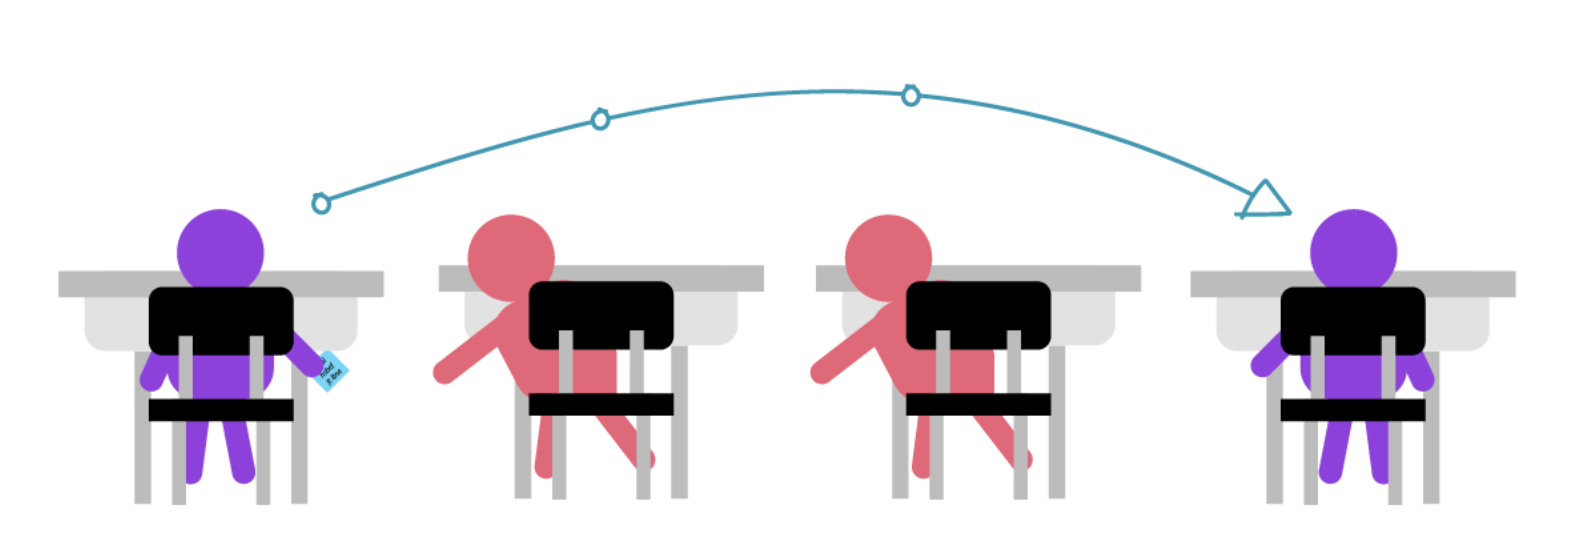
\includegraphics[scale=0.5]{normal}
\end{center}

Nevertheless, this is nowhere close in providing ample assurance on the security of the transmission as symmetric cryptography doesn't address the issue where someone could just eavesdrop and steal the symmetric key being sent from the sender to the receiver. \\

\begin{center}
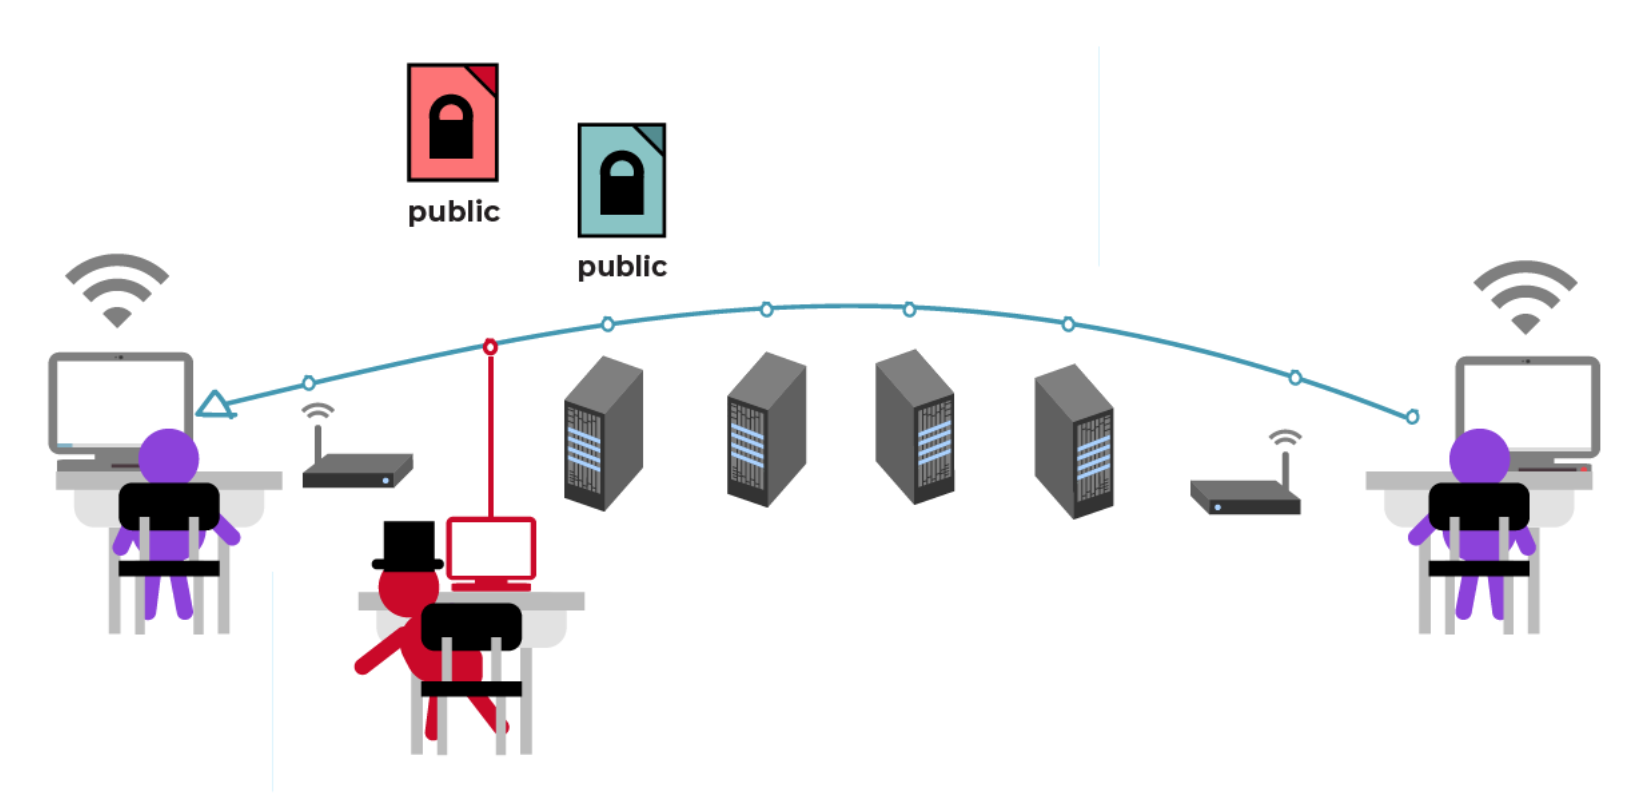
\includegraphics[scale=0.5]{midatk}
\end{center}

This allows the eavesdropper to conduct attacks in the middle by intercepting the message and make alterations to the contents. the attacker could read, alter and delete information packed in the payload and sends it to the receiver. \\
 
\begin{center}
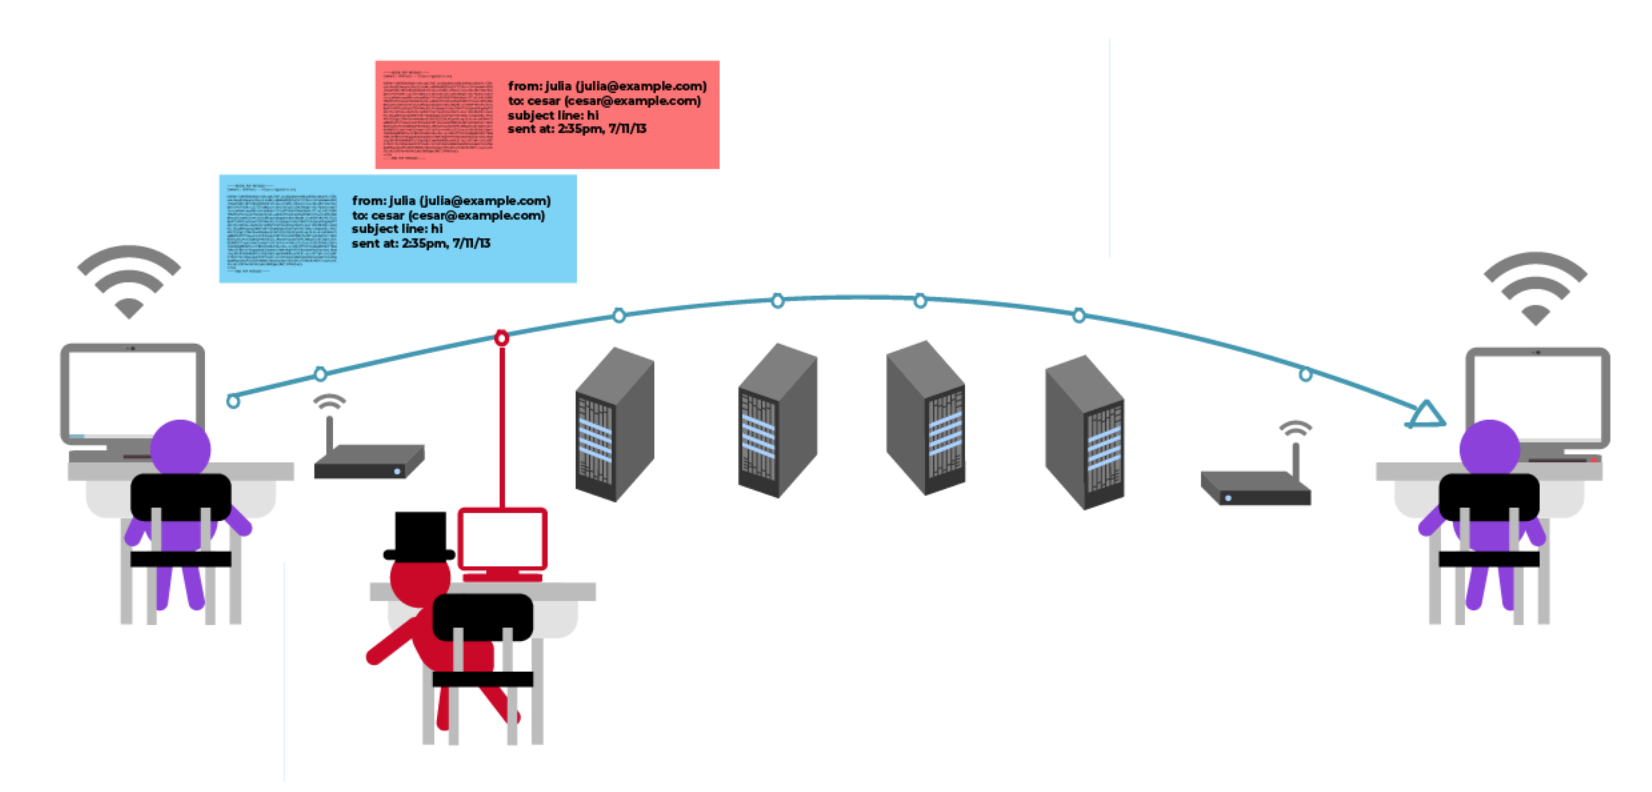
\includegraphics[scale=0.5]{messing}
\end{center}

Consequently, the wrong message will be directed towards the receiver instead. \\

\begin{center}
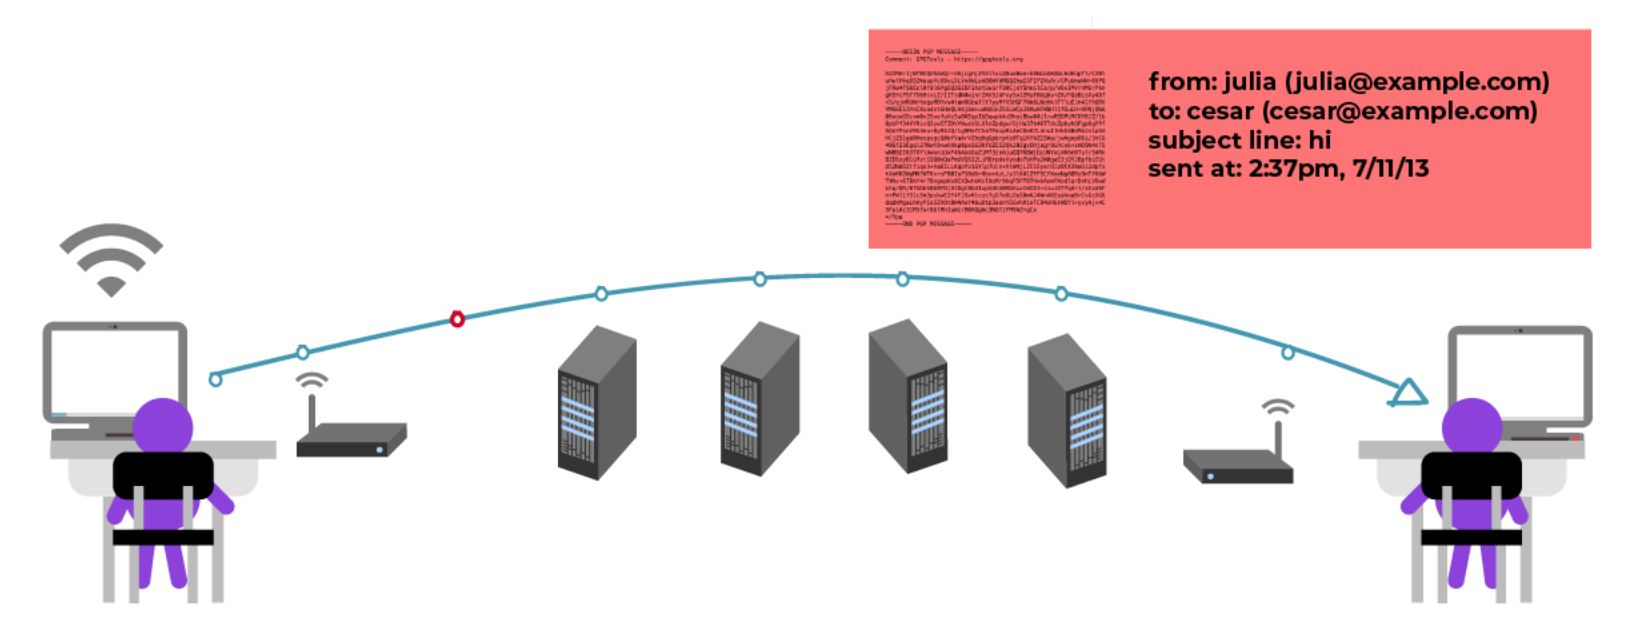
\includegraphics[scale=0.5]{wrong}
\end{center}

To compensate for this vulnerability, another encryption has to be implemented to make the symmetric key resilient to the attacks mentioned above. One initiative that can be resorted to is by encrypting the symmetric key using public key and read the decrypted version using the corresponding private key. The idea is to have the receiver broadcasting his or her public key while the sender use it to encrypt the keys or messages. As a result, only the intended can read the data while the intermediaries only have access to the metadata, such as the subject line, dates, sender, and recipient.\\

\begin{center}
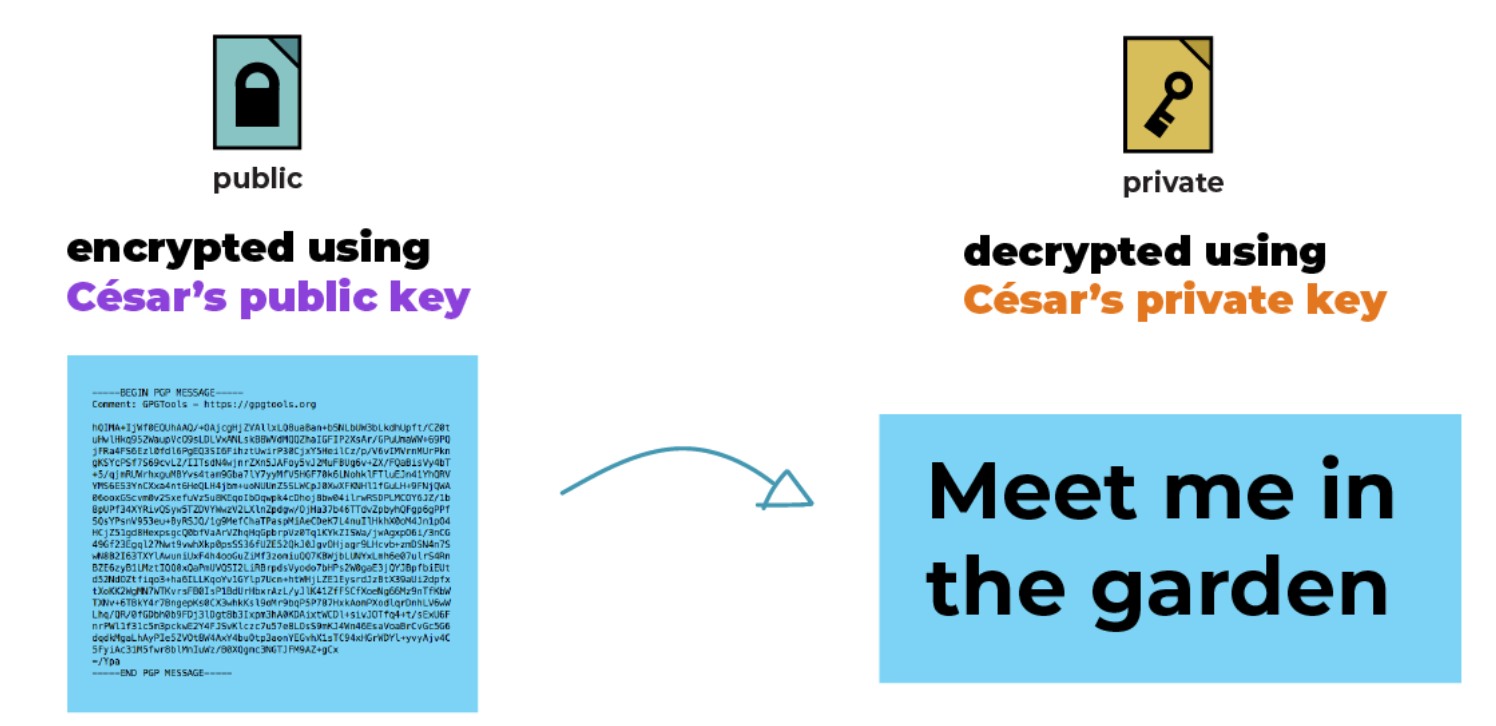
\includegraphics[scale=0.5]{proper}
\end{center}
\newpage
\section*{Purpose:}
The aim of this project is to develop a secure cloud storage application for Dropbox, Box, Google Drive, Office365 etc. For example, the application should be able to secure all files that are uploaded to the cloud, such that only people that are part of your “Secure Cloud Storage Group” will be able to decrypt your uploaded files. To all other users the files will be encrypted. \\ 

A suitable key management system will be designed and implemented for the application that will allow files to be shared securely, and users to be added and removed from “Secure Cloud Storage Group”. The application can be set up on a desktop or mobile platform and make use of any open source cryptographic libraries.
\section*{Design}
The implementation of this assignment can be divided into mainly two components: User Interface and a Cloud Storage Group. These components make use of different modules that consists of helper functions to execute their tasks. \\

The highlight of the design revolves around how to transmit symmetric keys to valid users in the group securely. The symmetric keys used for encryption when uploading files and decryption when downloading. One critical assumption that is took on during the development of the application is such that the activities of the cloud storage group is always being peeked on and the contents in it is always exposed to outsiders. \\

As a result, the contents in the cloud storage has to be encrypted for data protection and can only be decrypted by users who have access to the symmetric keys. To achieve this, a symmetric key has to shared securely among the users. The initiative taken here is to have the users send their public keys to the cloud storage group, so that it can be used to encrypt the symmetric key during transmission. \\

For this assignment, the target cloud storage is Google Drive. Further and more circumstantial explanation of the modus operandi will be elaborated later while the described design is as illustrated below.
\begin{center}
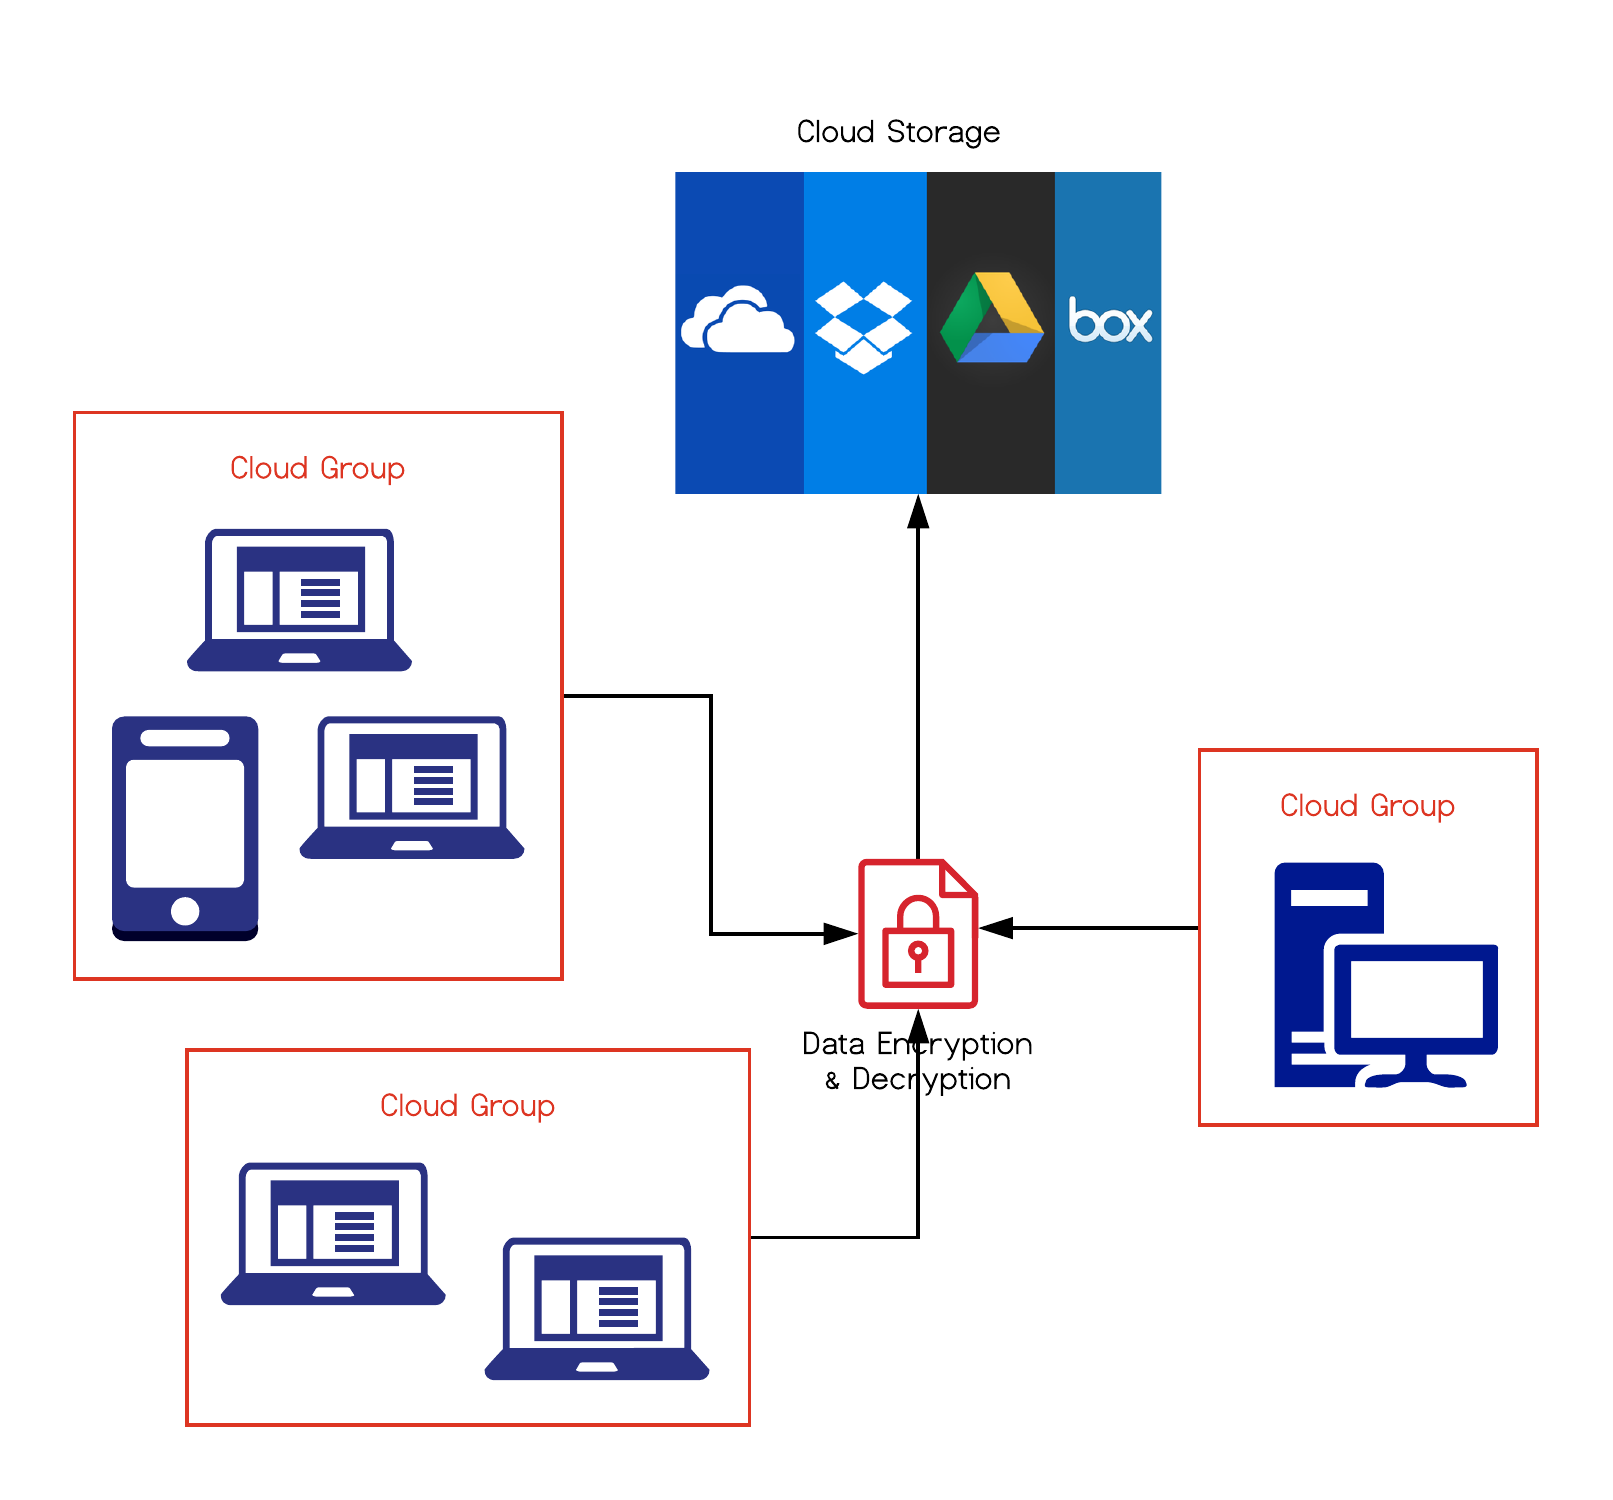
\includegraphics[scale=0.55]{design}
\end{center}
\newpage
\subsection*{User Interface}
\subsubsection*{Implementation:}
The user interface allows every user to log in using their user names and create their own unique asymmetrical keys. The asymmetrical keys of every user is stored, so that it can loaded the next time the same users access the user interface. Each asymmetrical key pair consist of a public key and a private key. The public key is sent along with the user name and the user port number to the cloud drive group as authentication terms to request for the symmetric key used for encryption and decryption of files in the group. If the user is not listed as one of legitimate members in the group, no symmetrical keys will be sent in response and an illegal trespassing exception will be reported. On the other hand, if the request is authorized, the public key sent will be utilized to encrypt the symmetric key and the package will then be transmitted back as response. \\

Subsequently, upon attaining the encrypted symmetric key from the cloud storage group, the private key in the key pair is then used to decrypt the encrypted symmetric key. To summarise, the symmetric key ensures the overall protection of the files in the cloud storage while its sanctity is assured by the asymmetrical key pairs approach used during transmissions. All users have to continuously request for the symmetrical keys from the cloud storage group to ensure they have the most updated version key in case of renewals being carried out due to a member being ousted.\\

A local GoogleDrive web server is then set up to handle authentication to the target folder in the cloud drive, before creating a GoogleDrive instance to enable any alterations to be done between local and the cloud drive. This allow the users to upload and download files from the cloud storage. During uploading, the symmetrical keys are used to encrypt the file contents before being written to the new file. Similarly, when downloading, the file contents read will be decrypted using the same key and written to file before being saved to the downloads folder. The application always assume that the visibility of the cloud storage is always compromised, so even if a non-member user managed to gain access to the files on the drive, he or she won't be able to read the file contents since he or she doesn't have access to the symmetric keys used in encryption and decryption. \\

The user class make use of the Key Manager module to create, save and load the users' corresponding keys, while all the encryption and decryption work are facilitated by importing the Encryptor module. Moreover, a socket is set up to relay requests to the cloud storage group whereas a listener is initialize to receive responses. 
\newpage
\subsubsection*{Code:}
\lstinputlisting[language=Python]{../User.py}
\newpage
\subsection*{Cloud Storage Group}
\subsubsection*{Implementation:}
The cloud storage group is mainly responsible for the management of the operations of the cloud storage such as adding or removing users from the members list, re-encrypting all the files on the drive folder when a user is evicted, listen to requests from users that are either members or non-members and relay the appropriate response message. \\

Upon activation, the cloud storage group will attempt to load a stored list into a set data structure which contains the user names of registered members. This is later used to validate the access of symmetrical keys when requested by users. Then, the symmetrical keys are loaded from the local data storage or created if no copy exists and stored for future usage and reference. \\ 

The cloud storage group employs the functionality of listener and clients from the multiprocessing library in Python. Multiprocessing is a package that supports spawning processes using an API similar to the threading module. The multiprocessing package offers both local and remote concurrency to the design. A listener, which is a wrapper for a bound socket is used to ‘listen’ for connections established by sockets from users. An authentication key is also used as the secret key here for an HMAC-based authentication challenge. This ensures that the connection can only be carried by users through the specified interface. \\

While active. the listener will attempt to receive requests from users through the connections established. These requests come in the form of a list containing the user names, address of user's listener and a public key. The cloud storage group will then respond by validating the user's membership using the member list. A illegal access error exception will be raised if a non-member attempts to request for the symmetrical key. On the contrary, if a member requests is authorised, a socket, i.e. Client will be used instead to set up a connection to the member's listener. The connection will serve as a pathway to transmit a symmetric key encrypted using the received public key back to the user. \\

For this component, the main concern that has to be take into account is a situation where a member is evicted, since adding a new member only involves the member having access to the symmetric key the next time he applies for it. In situation where a member is removed from the list, it is essential to have counter measures designated for it. There are two alternatives available for this complexity. Either the Cloud Storage Group could broadcast the new symmetric key to every members in the user list or it could just wait for an incoming request for symmetric keys from its group members and send the new ones during the transmissions. In this context, the latter is selected to as there would be no need for new symmetrical keys if no upload or download activities are carried out by the users, hence unnecessary broadcasting can be avoided, thus reducing the complexity of the routine algorithm. \\

Knowing that, the only protocols needed when a member is removed from the group are as follows:
\begin{itemize}
\item Decrypt all the files in the corresponding cloud drive.
\item Create a new symmetric key and save the key.
\item Encrypt all the files in the corresponding cloud drive.
\end{itemize}
The mentioned steps are crucial and requisite to avoid the removed member from having access to the drive and being able to read the contents of the uploaded files on the drive. A shared lock used to prevent transmissions and substituting of symmetric key in the group.
\vspace*{10mm}
\subsubsection*{Code:}
\lstinputlisting[language=Python]{../CloudGroup.py}
\newpage
\section*{Modules}
Since a lot of subroutines that leverage available cryptography libraries are shared by both classes mentioned above, modules are created for different purposes to provide helper functions while significantly reducing the need to import corresponding cryptographic libraries in every classes aside from repeating the same chunk of code. \\
\subsection*{Encryptor}
\subsubsection*{Implementation}
The Encryptor is set up to process all the encryption and decryption of the files passed. This module uses Fernet since it guarantees that a text encrypted by it cannot be manipulated or read without the specific passed key. Fernet is known for its symmetric authenticated cryptography implementation(also known as “secret key”). \\

Helper functions included in this module are:
\begin{itemize}
\item generating a fresh Fernet key.
\item generating a private, 2048 bits long RSA key which unlike keys used in symmetric cryptography, has a complex internal structure with specific mathematical properties.
\item encrypt a plain text using the passed key and return the encrypted version
\item decrypt an encrypted text using the passed key and  return the decrypted version
\end{itemize} 
\vspace*{10mm}
\subsubsection*{Code:}
\lstinputlisting[language=Python]{../Encryptor.py}
\newpage
\subsection*{Drive Manager}
\subsubsection*{Implementation}
The Drive Manager is a simple module that provides simple functionalities such as encrypting, decrypting, listing and deleting all the files in the corresponding folder. This module is built upon the Encryptor. 
\vspace*{10mm}
\subsubsection*{Code:}
\lstinputlisting[language=Python]{../DriveManager.py}
\newpage
\subsection*{Key Manager}
\subsubsection*{Implementation}
The Key Saver is a module responsible for key management. It takes advantage of the subroutines available in the Cryptography libraries to implement its functions:
\begin{itemize}
\item saving private key by converting it into bytes form using serialization and writing the contents onto a file.
\item load private key by reading the byte form contents of the passed file.
\item Extracting the public part of a key in bytes.
\item Generate a symmetric key using SHA-256, a cryptographic secure hash algorithm 
\end{itemize}
\vspace*{10mm}
\subsubsection*{Code:}
\lstinputlisting[language=Python]{../KeySaver.py} 
\vspace*{30mm}
\section*{Improvements:}
In long run, a graphical user interface version of the application can be developed to provide more comprehensive usage and systematic interactive usage to users. Better threads and lock management for the program. Moreover, a master server class can be implemented to regulate all the  contents and traffic data on the cloud storage. As for the encryption, signing and verification can be implemented externally to prevent impostor from stealing the public key in asymmetric encryption. 
\end{document}